% Use a package to avoid old (La)TeX habits.
\RequirePackage[l2tabu, orthodox]{nag}

% jsarticle: improved version of Japanese article style
% [dvipdfmx]: we use dvipdfmx.
% [uplatex]: we use uplatex.
% [papersize]: tell page size to pdf generator.
% [a4paper]: paper size is A4.
% [10pt]: point size is 10pt.
\documentclass[dvipdfmx,uplatex,papersize,a4paper,10pt]{jsarticle}

% This file is UTF-8 encoded.
\usepackage[utf8]{inputenc}
% Use T1 instead of OT1 for European texts.
\usepackage[T1]{fontenc}
% Fix Computer Modern rounding. Use this if you don't want to use Latin Modern.
% \usepackage{fix-cm}
% Use Latin Modern instead of Computer Modern font.
\usepackage{lmodern}

% AMS-related packages
\usepackage{amstext,amsmath,amsthm,amssymb,amsfonts}

% Avoid non-AMS mathematical usage.
\usepackage[all, warning]{onlyamsmath}

% Use otf fonts.
\usepackage{otf}
% Avoid "Font Shape undefined" error for italic Japanese texts.
\DeclareFontShape{JY2}{hmc}{m}{it}{<->ssub*hmc/m/n}{}
\DeclareFontShape{JY2}{hmc}{m}{sl}{<->ssub*hmc/m/n}{}
\DeclareFontShape{JY2}{hmc}{m}{sc}{<->ssub*hmc/m/n}{}
\DeclareFontShape{JY2}{hgt}{m}{it}{<->ssub*hgt/m/n}{}
\DeclareFontShape{JY2}{hgt}{m}{sl}{<->ssub*hgt/m/n}{}
\DeclareFontShape{JY2}{hmc}{bx}{it}{<->ssub*hgt/m/n}{}
\DeclareFontShape{JY2}{hmc}{bx}{sl}{<->ssub*hgt/m/n}{}
\DeclareFontShape{JT2}{hmc}{m}{it}{<->ssub*hmc/m/n}{}
\DeclareFontShape{JT2}{hmc}{m}{sl}{<->ssub*hmc/m/n}{}
\DeclareFontShape{JT2}{hmc}{m}{sc}{<->ssub*hmc/m/n}{}
\DeclareFontShape{JT2}{hgt}{m}{it}{<->ssub*hgt/m/n}{}
\DeclareFontShape{JT2}{hgt}{m}{sl}{<->ssub*hgt/m/n}{}
\DeclareFontShape{JT2}{hmc}{bx}{it}{<->ssub*hgt/m/n}{}
\DeclareFontShape{JT2}{hmc}{bx}{sl}{<->ssub*hgt/m/n}{}

% Use newtx fonts; maybe should be avoided in paper submissions.
\usepackage{newtxtext,newtxmath}

% Scale bigops in math. Not needed if we use newtxmath.
% \usepackage{exscale}

% \braket{}, \set{}
\usepackage{braket}

% Japanese Ruby generation.
\usepackage{pxrubrica}

% Syntax-highlighted program listings.
% jlisting: allow Japanese text in listings.
\usepackage{listings}

% Pass pagesize to DVI and configure page layout.
% [pass] is used to disable page layout overriding. Remove it if you want to configure page layout through this package.
% [dvipdfm] is for dvipdfmx.
% \usepackage[dvipdfm,pass]{geometry}

% Extended graphics package; provides \includegraphics.
\usepackage{graphicx}

% Extended color package; provides \color.
\usepackage{xcolor}

% Provides \url.
\usepackage{url}

% \mleft/\mright, a little clever replacements for \left/\right.
\usepackage{mleftright}

% \mathscr
\usepackage{mathrsfs}
% Override ursfs.fd to suppress "Font shape `U/rsfs/m/n' in size <5.5>/<10.5> not available" warning.
\DeclareFontFamily{U}{rsfs}{\skewchar\font127}
\DeclareFontShape{U}{rsfs}{m}{n}{%
  % <5> <6> rsfs5
  <5> <5.5> <6> rsfs5
  <7> rsfs7
  % <8> <9> <10> <10.95> <12> <14.4> <17.28> <20.74> <24.88> rsfs10
  <8> <9> <10> <10.5> <10.95> <12> <14.4> <17.28> <20.74> <24.88> rsfs10
}{}

% Part of hyperref.
\usepackage{nameref}

% Turns almost everything into hyper-reference.
\usepackage{hyperref}
% Improves non-ASCII characters in bookmarks.
\usepackage{pxjahyper}

% Float wrapper for algorithms.
\usepackage{algorithm}
% One of algorithm typesetting environments.
\usepackage{algpseudocode}

% Provides \cref, which automatically emits Lemma, Definition, etc.
\usepackage{cleveref}

\usepackage{tikz}
\usetikzlibrary{positioning,babel,arrows}

\theoremstyle{definition}
\newtheorem{definition}{定義}[section]
\newtheorem{example}[definition]{例}
\newtheorem{theorem}[definition]{定理}
\newtheorem{lemma}[definition]{補題}
\newtheorem{corollary}[definition]{系}
\newtheorem{proposition}[definition]{命題}
\newtheorem{axiom}[definition]{公理}
\newtheorem{remark}[definition]{注意}
\newtheorem{exercise}{練習問題}[section]

\crefname{definition}{定義}{定義}
\Crefname{definition}{定義}{定義}
\crefname{example}{例}{例}
\Crefname{example}{例}{例}
\crefname{theorem}{定理}{定理}
\Crefname{theorem}{定理}{定理}
\crefname{lemma}{補題}{補題}
\Crefname{lemma}{補題}{補題}
\crefname{corollary}{系}{系}
\Crefname{corollary}{系}{系}
\crefname{proposition}{命題}{命題}
\Crefname{proposition}{命題}{命題}
\crefname{axiom}{公理}{公理}
\Crefname{axiom}{公理}{公理}
\crefname{remark}{注意}{注意}
\Crefname{remark}{注意}{注意}
\crefname{exercise}{練習問題}{練習問題}
\Crefname{exercise}{練習問題}{練習問題}

\DeclareMathOperator{\id}{id}
\DeclareMathOperator{\Alg}{Alg}
\DeclareMathOperator{\Coalg}{Coalg}
\DeclareMathOperator{\RCA}{RCA}
\DeclareMathOperator{\CRA}{CRA}

\title{再帰的余代数いろいろ}
\author{原 将己}
%\date{2017年01月13日}

\begin{document}

\maketitle

\section{代数と余代数}

以下、 $\mathbf{C}$は圏とし、$F \colon \mathbf{C} \to \mathbf{C}$ は自己関手とする。

\begin{definition}[代数、余代数]

  $C$ の対象と射の組 $(A, \alpha)$ であって $\alpha \colon FA \to A$ となるものを \emph{$F$-代数 ($F$-algebra)} と呼ぶ。

  $C$ の対象と射の組 $(A, \alpha)$ であって $\alpha \colon A \to FA$ となるものを \emph{$F$-余代数 ($F$-coalgebra)} と呼ぶ。

  $F$-代数 $(A, \alpha)$ から $(B, \beta)$ への準同型とは、 $h \colon A \to B$ であって $\beta \circ Fh = h \circ \alpha$ となるもののことである。 $F$-代数とその準同型のなす圏を $\Alg(F)$ と書く。

  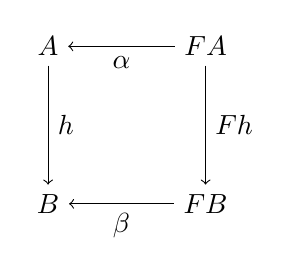
\begin{tikzpicture}[auto,every node/.style={on grid,node distance=2cm}]
    \node (A) {$A$};
    \node[right of=A] (FA) {$FA$};
    \node[below of=A] (B) {$B$};
    \node[right of=B] (FB) {$FB$};
    \draw[->] (FA) -- node {$\alpha$} (A);
    \draw[->] (FB) -- node {$\beta$} (B);
    \draw[->] (A) -- node {$h$} (B);
    \draw[->] (FA) -- node {$Fh$} (FB);
  \end{tikzpicture}

  $F$-余代数 $(A, \alpha)$ から $(B, \beta)$ への準同型とは、 $h \colon A \to B$ であって $\beta \circ h = Fh \circ \alpha$ となるもののことである。 $F$-余代数とその準同型のなす圏を $\Coalg(F)$ と書く。

  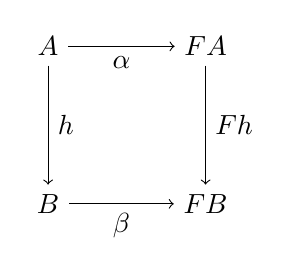
\begin{tikzpicture}[auto,every node/.style={on grid,node distance=2cm}]
    \node (A) {$A$};
    \node[right of=A] (FA) {$FA$};
    \node[below of=A] (B) {$B$};
    \node[right of=B] (FB) {$FB$};
    \draw[->] (A) -- node[swap] {$\alpha$} (FA);
    \draw[->] (B) -- node[swap] {$\beta$} (FB);
    \draw[->] (A) -- node {$h$} (B);
    \draw[->] (FA) -- node {$Fh$} (FB);
  \end{tikzpicture}
\end{definition}

\begin{definition}[余代数-代数準同型]
  $F$-余代数 $(A, \alpha)$ から $F$-代数 $(B, \beta)$ への\emph{余代数-代数準同型 (coalgebra-to-algebra homomorphism)} とは、 $h \colon A \to B$ であって、 $\beta \circ Fh \circ \alpha = h$ となるもののことである。

  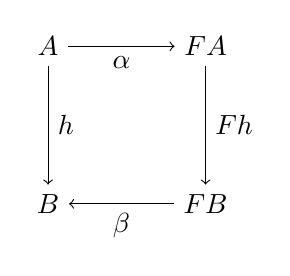
\begin{tikzpicture}[auto,every node/.style={on grid,node distance=2cm}]
    \node (A) {$A$};
    \node[right of=A] (FA) {$FA$};
    \node[below of=A] (B) {$B$};
    \node[right of=B] (FB) {$FB$};
    \draw[->] (A) -- node[swap] {$\alpha$} (FA);
    \draw[->] (FB) -- node {$\beta$} (B);
    \draw[->] (A) -- node {$h$} (B);
    \draw[->] (FA) -- node {$Fh$} (FB);
  \end{tikzpicture}
\end{definition}

\begin{definition}[始代数と終余代数]
  $\Alg(F)$ の始対象を\emph{始代数 (initial algera)}という。$\Coalg(F)$ の終対象を\emph{終余代数 (terminal coalgebra, final coalgebra)}という。

  定義より、始代数と終余代数は(存在するならば)同型を除いて一意である。
\end{definition}

\begin{definition}[再帰的余代数と余再帰的代数]

  余代数であって、任意の代数への準同型が一意に存在するものを\emph{再帰的$F$-余代数 (recursive $F$-coalgebra)}という。本資料では再帰的余代数からなる$\Coalg(F)$の充満部分圏を$\RCA(F)$と表記する。

  代数であって、任意の余代数からの準同型が一意に存在するものを\emph{余再帰的$F$-代数 (corecursive $F$-algebra)}という。本資料では余再帰的代数からなる$\Alg(F)$の充満部分圏を$\CRA(F)$と表記する。
\end{definition}

\begin{remark}
  再帰的余代数と始代数の普遍性は良く似ている。実際、 $\alpha$ が可逆のとき、この2つの定義は ($\alpha$ の向きを互いに逆にすることで) 同値になる。

  同様に、余再帰的代数と終余代数の定義も、 $\alpha$ が可逆のときに同値になる。
\end{remark}

\section{Lambekの定理}

\begin{theorem}[Lambek]
  始代数 $(A, \alpha)$ の $\alpha$ は常に可逆である。双対的に、終余代数も可逆である。
\end{theorem}

\begin{proof}
  始代数について示す。 $(A, \alpha)$ を始代数とする。このとき $(FA, F\alpha)$ も代数だから、代数の準同型 ($h \colon A \to FA$ であって $F\alpha \circ Fh = h \circ \alpha$ となるもの)が存在する。

  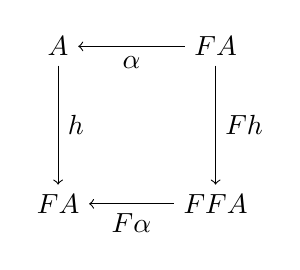
\begin{tikzpicture}[auto,every node/.style={on grid,node distance=2cm}]
    \node (A) {$A$};
    \node[right of=A] (FA) {$FA$};
    \node[below of=A] (FA2) {$FA$};
    \node[right of=FA2] (FFA2) {$FFA$};
    \draw[->] (FA) -- node {$\alpha$} (A);
    \draw[->] (FFA2) -- node {$F\alpha$} (FA2);
    \draw[->] (A) -- node {$h$} (FA2);
    \draw[->] (FA) -- node {$Fh$} (FFA2);
  \end{tikzpicture}

  $h$ も $\alpha$ も代数の準同型だから、 $\alpha \circ h$ は $(A, \alpha)$ の自己準同型である。一方、 $\id_A$ も $(A, \alpha)$ の自己準同型である。始代数からの準同型は一意だから、 $\alpha \circ h = \id_A$ である。

  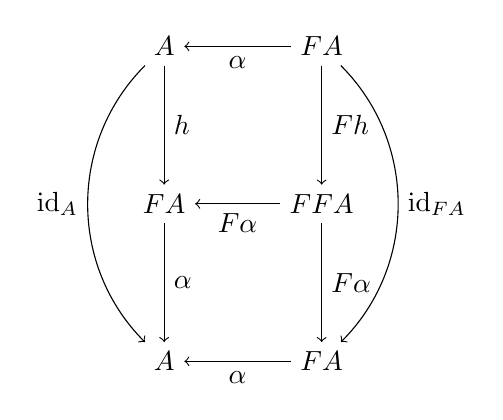
\begin{tikzpicture}[auto,every node/.style={on grid,node distance=2cm}]
    \node (A) {$A$};
    \node[right of=A] (FA) {$FA$};
    \node[below of=A] (FA2) {$FA$};
    \node[right of=FA2] (FFA2) {$FFA$};
    \node[below of=FA2] (A3) {$A$};
    \node[right of=A3] (FA3) {$FA$};
    \draw[->] (FA) -- node {$\alpha$} (A);
    \draw[->] (FFA2) -- node {$F\alpha$} (FA2);
    \draw[->] (FA3) -- node {$\alpha$} (A3);
    \draw[->] (A) -- node {$h$} (FA2);
    \draw[->] (FA) -- node {$Fh$} (FFA2);
    \draw[->] (FA2) -- node {$\alpha$} (A3);
    \draw[->] (FFA2) -- node {$F\alpha$} (FA3);
    \draw[->] (A) to[bend right=45] node[swap] {$\id_A$} (A3);
    \draw[->] (FA) to[bend left=45] node {$\id_{FA}$} (FA3);
  \end{tikzpicture}

  $\alpha \circ h = \id_A$ と $h$ の準同型性により、 $h \circ \alpha = F\alpha \circ Fh = F\id_A = \id_{FA}$ である。

  したがって、 $h$ は $\alpha$ の逆射である。
\end{proof}

\begin{corollary}
  始代数(の逆射)は再帰的余代数である。双対的に、終余代数(の逆射)は余再帰的代数である。
\end{corollary}

\begin{theorem}
  始代数(の逆射)は$\RCA(F)$の終対象である。双対的に、終余代数(の逆射)は$\CRA(F)$の始対象である。
\end{theorem}

\begin{proof}
  $(A, \alpha)$ を始代数とする。このとき $(A, \alpha^{-1})$が$\RCA(F)$の終対象であることを示す。

  $(B, \beta) \in \RCA(F)$ とする。 $(B, \beta)$ から $(A, \alpha^{-1})$ への代数準同型は、$(B, \beta)$ から $(A, \alpha)$ への余代数-代数準同型に他ならない。したがって $B$ の再帰性から、代数準同型は一意である。

  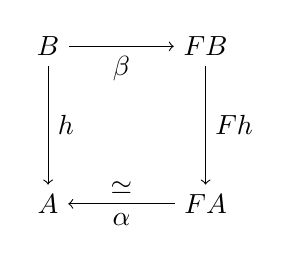
\begin{tikzpicture}[auto,every node/.style={on grid,node distance=2cm}]
    \node (A) {$A$};
    \node[right of=A] (FA) {$FA$};
    \node[above of=A] (B) {$B$};
    \node[right of=B] (FB) {$FB$};
    \draw[->] (FA) -- node {$\alpha$} node[swap] {$\simeq$} (A);
    \draw[->] (B) -- node[swap] {$\beta$} (FB);
    \draw[->] (B) -- node {$h$} (A);
    \draw[->] (FB) -- node {$Fh$} (FA);
  \end{tikzpicture}
\end{proof}

\section{逆Lambekの定理}

(逆Lambekという名前は本資料に固有である。)

\begin{lemma}
  $(A, \alpha)$ が再帰的余代数であるとき、 $(FA, F\alpha)$ も再帰的余代数である。双対的に、 $(A, \alpha)$ が余再帰的代数であるとき、 $(FA, F\alpha)$ も余再帰的代数である。
\end{lemma}

\begin{proof}
  $(A, \alpha)$ を再帰的余代数とし、 $(B, \beta)$ を代数とする。

  $A$ の再帰性より、 $A$ から $B$ への余代数-代数準同型 ($h \colon A \to B$ であって $\beta \circ Fh \circ \alpha = h$ となるもの) が一意に存在する。これを用いて $f = \beta \circ Fh$ と定義する。

  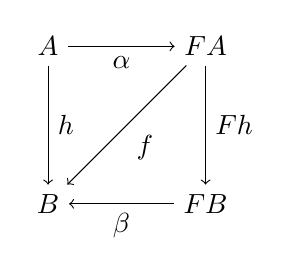
\begin{tikzpicture}[auto,every node/.style={on grid,node distance=2cm}]
    \node (A) {$A$};
    \node[right of=A] (FA) {$FA$};
    \node[below of=A] (B) {$B$};
    \node[right of=B] (FB) {$FB$};
    \draw[->] (A) -- node[swap] {$\alpha$} (FA);
    \draw[->] (FB) -- node {$\beta$} (B);
    \draw[->] (A) -- node {$h$} (B);
    \draw[->] (FA) -- node {$Fh$} (FB);
    \draw[->] (FA) -- node {$f$} (B);
  \end{tikzpicture}

  この $f$ は $\beta \circ Ff \circ F\alpha = \beta \circ F(\beta \circ Fh \circ \alpha) = \beta \circ Fh = f$ を満たす。したがって $f$ は $FA$ から $B$ への余代数-代数準同型である。

  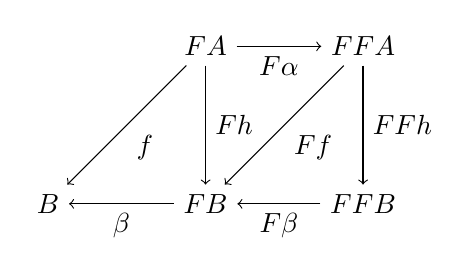
\begin{tikzpicture}[auto,every node/.style={on grid,node distance=2cm}]
    %\node (A) {$A$};
    \node (A) {};
    \node[right of=A] (FA) {$FA$};
    \node[right of=FA] (FFA) {$FFA$};
    \node[below of=A] (B) {$B$};
    \node[right of=B] (FB) {$FB$};
    \node[right of=FB] (FFB) {$FFB$};
    %\draw[->] (A) -- node[swap] {$\alpha$} (FA);
    \draw[->] (FA) -- node[swap] {$F\alpha$} (FFA);
    \draw[->] (FB) -- node {$\beta$} (B);
    \draw[->] (FFB) -- node {$F\beta$} (FB);
    %\draw[->] (A) -- node {$h$} (B);
    \draw[->] (FA) -- node {$Fh$} (FB);
    \draw[->] (FFA) -- node {$FFh$} (FFB);
    \draw[->] (FA) -- node {$f$} (B);
    \draw[->] (FFA) -- node {$Ff$} (FB);
  \end{tikzpicture}

  逆に $f' \colon FA \to B$ が $\beta \circ Ff' \circ F\alpha = f'$ を満たすとする。 $h' = f' \circ \alpha$ とおくと、 $\beta \circ Fh' \circ \alpha = \beta \circ Ff' \circ F\alpha \circ \alpha = f' \circ \alpha = h'$ となるから、 $h'$ は $A$ から $B$ への余代数-代数準同型である。

  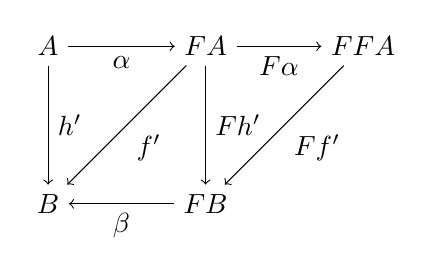
\begin{tikzpicture}[auto,every node/.style={on grid,node distance=2cm}]
    \node (A) {$A$};
    \node[right of=A] (FA) {$FA$};
    \node[right of=FA] (FFA) {$FFA$};
    \node[below of=A] (B) {$B$};
    \node[right of=B] (FB) {$FB$};
    %\node[right of=FB] (FFB) {$FFB$};
    \draw[->] (A) -- node[swap] {$\alpha$} (FA);
    \draw[->] (FA) -- node[swap] {$F\alpha$} (FFA);
    \draw[->] (FB) -- node {$\beta$} (B);
    %\draw[->] (FFB) -- node {$F\beta$} (FB);
    \draw[->] (A) -- node {$h'$} (B);
    \draw[->] (FA) -- node {$Fh'$} (FB);
    %\draw[->] (FFA) -- node {$FFh'$} (FFB);
    \draw[->] (FA) -- node {$f'$} (B);
    \draw[->] (FFA) -- node {$Ff'$} (FB);
  \end{tikzpicture}

  $A$ の再帰性から $h' = h$ となる。したがって、 $f' = \beta \circ Ff' \circ F\alpha = \beta \circ Fh' = \beta \circ Fh = f$ となる。

  以上より $FA$ から $B$ への余代数-代数準同型は一意に存在する。したがって、 $(FA, F\alpha)$ は再帰的余代数である。
\end{proof}

\begin{theorem}[逆Lambek]
  $\RCA(F)$ の終対象は可逆である。双対的に、 $\CRA(F)$ の始対象は可逆である。
\end{theorem}

\begin{proof}
  $(A, \alpha)$ を $\RCA(F)$ の終対象とする。$(FA, F\alpha)$ も再帰的余代数だから、 $(A, \alpha)$ の終性より、$FA$ から $A$ への余代数準同型 ($h \colon FA \to A$ であって $\alpha \circ h = Fh \circ F\alpha$ となるもの) が存在する。

  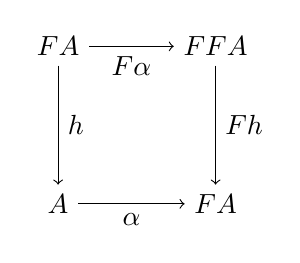
\begin{tikzpicture}[auto,every node/.style={on grid,node distance=2cm}]
    \node (A) {$A$};
    \node[right of=A] (FA) {$FA$};
    \node[above of=A] (FA2) {$FA$};
    \node[right of=FA2] (FFA2) {$FFA$};
    \draw[->] (A) -- node[swap] {$\alpha$} (FA);
    \draw[->] (FA2) -- node[swap] {$F\alpha$} (FFA2);
    \draw[->] (FA2) -- node {$h$} (A);
    \draw[->] (FFA2) -- node {$Fh$} (FA);
  \end{tikzpicture}

  $h$ も $\alpha$ も余代数の準同型だから、 $h \circ \alpha$ は $(A, \alpha)$ の自己準同型である。一方、 $\id_A$ も $(A, \alpha)$ の自己準同型である。終再帰的余代数への準同型は一意だから、 $h \circ \alpha = \id_A$ である。

  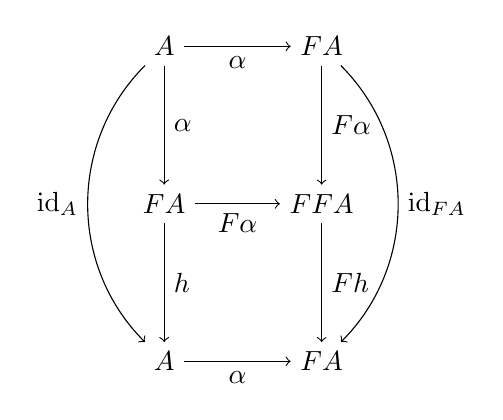
\begin{tikzpicture}[auto,every node/.style={on grid,node distance=2cm}]
    \node (A) {$A$};
    \node[right of=A] (FA) {$FA$};
    \node[above of=A] (FA2) {$FA$};
    \node[right of=FA2] (FFA2) {$FFA$};
    \node[above of=FA2] (A3) {$A$};
    \node[right of=A3] (FA3) {$FA$};
    \draw[->] (A) -- node[swap] {$\alpha$} (FA);
    \draw[->] (FA2) -- node[swap] {$F\alpha$} (FFA2);
    \draw[->] (A3) -- node[swap] {$\alpha$} (FA3);
    \draw[->] (FA2) -- node {$h$} (A);
    \draw[->] (FFA2) -- node {$Fh$} (FA);
    \draw[->] (A3) -- node {$\alpha$} (FA2);
    \draw[->] (FA3) -- node {$F\alpha$} (FFA2);
    \draw[->] (A3) to[bend right=45] node[swap] {$\id_A$} (A);
    \draw[->] (FA3) to[bend left=45] node {$\id_{FA}$} (FA);
  \end{tikzpicture}

  $h \circ \alpha = \id_A$ と $h$ の準同型性により、 $\alpha \circ h = Fh \circ F\alpha = F\id_A = \id_{FA}$ である。

  したがって、 $h$ は $\alpha$ の逆射である。
\end{proof}

\begin{corollary}
  $\RCA(F)$ の終対象(の逆射)は始代数である。双対的に、$\CRA(F)$ の始対象(の逆射)は終余代数である。
\end{corollary}

\bibliographystyle{plain}
\bibliography{refs}

\end{document}

